\section{The FOCUSA Backend}

The FOCUSA backend is one of the many deliverables our project delivers.
Initially, we broke each "service" our project delivers into isolated, 
horizontally scalable and loosely coupled architecture. 
Called the microservice architecture, it breaks code into small and 
manageable pieces which can be rapidly implemented and quickly tested.
It is important to note that I will be swapping between the terms microservice 
and service very often. When I say service, I mean microservice.

Each microservice runs in a \textbf{highly isolated manner}, without needing to share
any resources in common. The services do not need to share any common memory, 
common variables, or common storage. \emph{How will services share data?} 
In case any services require to communicate with each other, they do so solely by 
message passing over WebSockets, or simple HTTP.

This architecture also supports \textbf{great scalability}. Each service, 
can run on it's own machine (in a containerised, virtual, physical, or 
even geographical manner) Thousands of instances of the same service can 
be spawned, and run independent of each other, governed by one or more load balancers.

Any communication with a microservice operates \textbf{over a stateless protocol}, 
like HTTP.
Typical to the TCP/IP suite, there isn't any specific full-duplex session maintenance 
protocol, and thus require a special token attached to every packet. This token is 
usually a random string of characters, referencing a session. The session could be 
managed by a specific service, but that would cause a centralised component, with a 
possible point of failure.

The approach we used was signing a \textbf{cryptographic token called a JWT (JSON Web Token)}. 
This token, generated by the authentication service is then attached by the client 
to every future request made to any other service. This is possible because the JWT contains 
ALL the session data as a JSON payload, encrypted and entrusted to the client. 
Session data is not stored between the services.

It is obviously risky to trust the client with storing session data. \emph{Can a client 
generate it's own JSON payload and impersonate a user?} No. (https://hasura.io/blog/best-practices-of-using-jwt-with-graphql/)

JWTs also contain a digital signature. Since all our services depend on the session state 
written in the JWT, shared by the client, we carefully adhered to these rules for handling 
JWTs throughout development:

\begin{itemize}
    \item Every JWT has a validity window, after which it expires. Always keep this window small. 
    Keeping a small window means that a JWT quickly expires after its creation, thus preventing 
    any malicious party from using the JWT for a long time.
    \item Every client also holds a session refresh cookie which is used to regenerate a JWT
    after expiry. The client will request for a new JWT without needing to login, by using the 
    refresh cookie.
    \item The JWT generation and refresh cookie session maintenance is done by the authentication 
    service.
\end{itemize}

Our approach uses an asymmetric key digital signature standard called RS256. Here, the authentication 
service signs the JWT using a private key. The public key is shared with all the other services. This 
way, the other services are able to verify the signature of the JWT shared by the client. As long as the 
JWT is signed by the private key owned by the authentication service, the other services will accept it. 
Failure to provide a valid JWT will lead to denial of service, since the service will assume a malicious 
user is playing with the system.

As listed in the Design chapter, the FOCUSA backend contains the following major services:
\begin{itemize}
    \item \textbf{Auth:} performs the authentication process based on a username and password, and returns refresh cookies with a JWT.
    \item \textbf{Roles:}  returns the roles that a user belongs to. It depicts the different roles that different admins perform.
    \item \textbf{Profiles:} Each user has a unique profile, containing details like the user display picture, username, and the various courses the user has subscribed to.
    \item \textbf{Courses:}  returns the details of the courses which includes the course title and the different users subscribed to the course, as well as a provision for new users to subscribe to the course. Only users with certain roles can moderate their respective courses.
    \item \textbf{Posts:} refers to posts posted by the course moderators. The moderators are able to perform CRUD operations on these posts
    \item \textbf{Notifications:}  sends notifications to the user devices and also monitors the database for changes.
    \item \textbf{Storage:} performs all functions related to file upload, download, and streaming.
\end{itemize}

The following sections will describe our workflow, and an overview on our deployment strategies.

\subsection{Workflow}

The task of building every service was decomposed into three main subtasks:
\begin{itemize}
    \item \textbf{DAO}, which includes a set of functions regarding Database, Analytics and Operations. 
    These functions are invoked and executed on call at the next stage.
    \item \textbf{REST API}, which acts as a thin ExpressJS layer between the main API gateway and the DAO.
    This layer performs RPC-based communication, with proper JWT verification checks.
    \item \textbf{GraphQL API gateway integration}, where the microservices are integrated, over a graph query language gateway.
    GraphQL API allows the developer to build surprisingly advanced systems by virtue of resolvers which invoke the REST API services.
    The GraphQL API gateway also supports queries, mutations, and subscriptions. This allows us to build practically any front-end, which 
    supports the typical query-response RPC-based mechanism, and also the more complex message-based notification mechanism.
\end{itemize}

\begin{figure}[h!]
    \begin{center}
        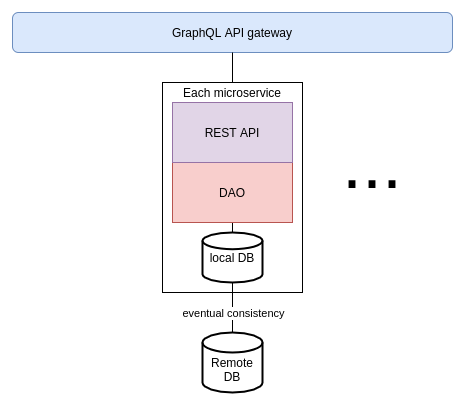
\includegraphics[width=8cm]{Microservice.png}
    \end{center}
    \caption{Our layered approach to building each microservice.}
    \label{fig:microservice}
\end{figure}

All members of the team have built at least one entire microservice, following this layered architecture for each service. 

It is important to note that our notification service was built using a pull-notification technique. This involves using a 
publisher-subscriber architecture which only transfers a digest of messages whenever the client asks for them. Unlike polling, 
this system operates on an event-loop.

\subsection{Deployment}

Initially we had decided to deploy it on the Heroku cloud. Heroku provides virtual containers, called dynos. Each free tier dyno 
by itself has very few resources allocated to it. An account is allowed to operate multiple dynos. Each service ran very efficiently, 
with latencies as low as 70ms per request.

We however quickly hit a roadblock when we realised that data isn't persisting at the dynos (See https://devcenter.heroku.com/articles/active-storage-on-heroku). 
Apparently, Heroku provides ephemeral storage to dynos. This means the storage is volatile, and gets purged after inactivity.
We need to integrate custom AWS S3 storage to the dyno if we want persistent storage. 

We ultimately decided to operate on self-hosted Docker containers. Docker was easier to customize and control. 
The only issue with self-hosting is server availablity. Hosting on AWS services is a long-term goal.